	\section {Análise léxica}
	
	Ferramentas que operam em código-fonte começam por transformar o código em um série de {\it tokens}, descartando recursos sem importância de o texto do programa, tais como espaços em branco ou comentários ao longo do caminho. A criação do fluxo de sinal é chamado de análise lexical. Regras léxicas muitas vezes usam expressões regulares para identificar fichas.
	Observa-se que a maioria dos {\it tokens} são representados inteiramente por seu tipo, mas para ser útil, o {\it tokens} de identificação requer uma peça adicional de informação: o nome do identificador. Para habilitar o relatório de erro útil mais tarde, os {\it tokens} devem transportar pelo menos um outro tipo de informação com eles: a sua posição no texto-fonte (geralmente um número de linha e um número de coluna). Para as mais simples ferramentas de análise estática, o trabalho está quase concluído neste ponto. Se toda a ferramenta tem que fazer é combinar os nomes de funções, o analisador pode ir através do fluxo de {\it tokens} procurando identificadores, combiná-los com uma lista de nomes de funções, e relatar o resultados.\\
	
	\section{Parser}
	
	Um analisador de linguagem usa uma gramática livre de contexto (CFG) para coincidir com os {\it tokens} correntes. A gramática é composta por um conjunto de produções que descrevem os símbolos (elementos) na língua. No Exemplo é enumerado um conjunto de produções que são capazes de analisar o fluxo de {\it tokens} de amostra.
	
	\begin{lstlisting}
	stmt := if_stmt | assign_stmt
	if_stmt := IF LPAREN expr RPAREN stmt
	expr := lval
	assign_stmt := lval EQUAL expr SEMI
	lval = ID | arr_access
	arr_access := ID arr_index+
	arr_idx := LBRACKET expr RBRACKET
	\end{lstlisting}
	
	O analisador executa uma derivação, combinando o fluxo de sinal contra as regras de produção. Se cada símbolo é ligado a partir da qual o símbolo foi derivado, uma árvore de análise é formada. Na Figura: \ref{fig:TreeParser} mostra uma árvore de análise criada, usando as regras de produção do exemplo anterior. Omiti-se terminais de símbolos que não carregam nomes \textit{(IF, LPAREN, RPAREN, etc.}), para fazer o principais características da árvore de análise mais óbvia.\\
	
	\clearpage
	\begin{figure}[h]
		\center
		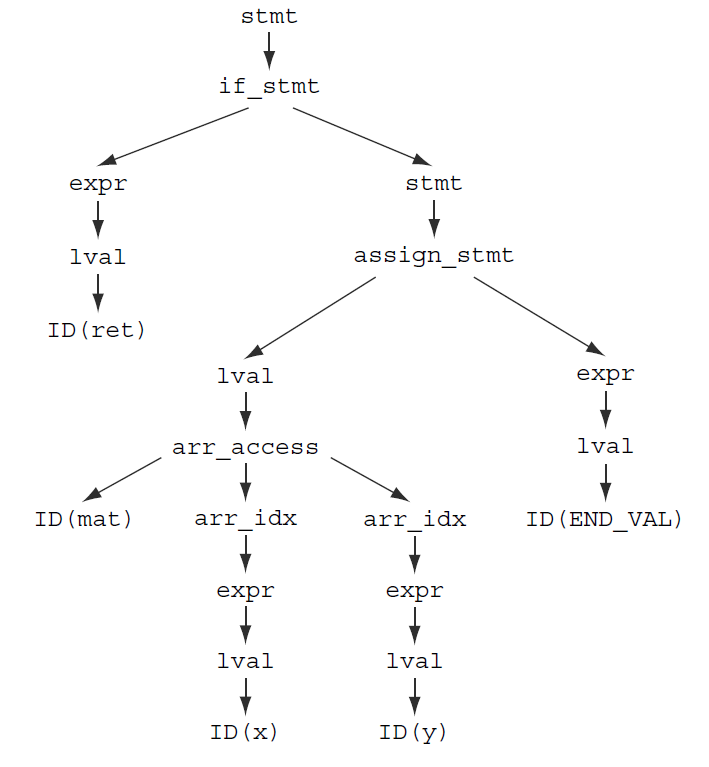
\includegraphics[width=0.8\textwidth]{Imagens/Arvore}
		\label{fig:TreeParser}
		\caption{Árvore de parser.}
	\end{figure}
	
	
	\subsection{Paser JDT Eclipse}
	No caso do \textit{parser} provido pela infraestrutura \textit{JDT} do eclipse,  a classe \textit{ASTParser} contida na biblioteca \textit{org.eclipse.jdt.core.dom} permite a criação de uma árvore de sintaxe abstrata.\\
	Este procedimento é realizado em todos os aquivos \textit{.java} contido em um projeto e com isso cada um possui uma referência de \textit{CompilationUnit} o qual permite acesso ao nó raiz árvore sintática de cada arquivo. O parse é gerado conforme as últimas definições da linguagem utilizando \textit{AST.JLS8}.\\ 
	\clearpage

	\begin{lstlisting}
		ASTParser parser = ASTParser.newParser(AST.JLS8);
		
		Map<String, String> options = JavaCore.getOptions();
		options.put(JavaCore.COMPILER_COMPLIANCE, JavaCore.VERSION_1_8);
		options.put(JavaCore.COMPILER_CODEGEN_TARGET_PLATFORM, JavaCore.VERSION_1_8);
		options.put(JavaCore.COMPILER_SOURCE, JavaCore.VERSION_1_8);
		
		parser.setKind(ASTParser.K_COMPILATION_UNIT);
		parser.setCompilerOptions(options);
		parser.setSource(contents);
		
		final CompilationUnit cu = (CompilationUnit) parser.createAST(null);
		return cu;
	\end{lstlisting}
	
	Neste, o \textit{parser} é realizado através de uma classe denominada de mesmo nome, a qual é instanciada um única vez no projeto através do padrão \textit{singleton} \cite{Gamma:1995:DPE:186897}.\\
	

	
	

	\section{Sintaxe abstrata}

	É possível fazer uma análise significativa em uma árvore de parser, e certos tipos de checagem estilísticas são mais bem executadas em uma árvore de análise, pois contém mais representações diretas do código assim como o programador escreve. No entanto, executar análise complexa em uma árvore de análise pode ser inconveniente. Os nós da árvore são derivados diretamente das regras de produção da gramática, e essas regras podem-se introduzir símbolos não terminais que existem apenas para fins de fazer a análise mais fácil e menos ambígua, ao invés de para o objetivo de produzir uma facilmente compreendido a árvore. É geralmente melhor para abstrair ambos os detalhes da gramática e as estruturas sintáticas presente no código fonte do programa. Uma estrutura de dados que faz estas coisas é chamado de uma árvore de sintaxe abstrata (AST). O objectivo da AST é fornecer uma versão padronizada do programa adequado para posteriores análises. A AST é normalmente construída associando código construção árvore com regras de produção da gramática. A Figura: \ref{fig:ArvoreAST} mostra uma AST. Observa-se que a instrução {\it if} agora tem uma outra ramificação vazia, o predicado testado pelo caso é agora uma comparação explícita para zero (o comportamento exigido pelo C), e acesso à matriz é uniformemente representada como uma operação de binário.\\
	
	\begin{figure}[h]
		\center
		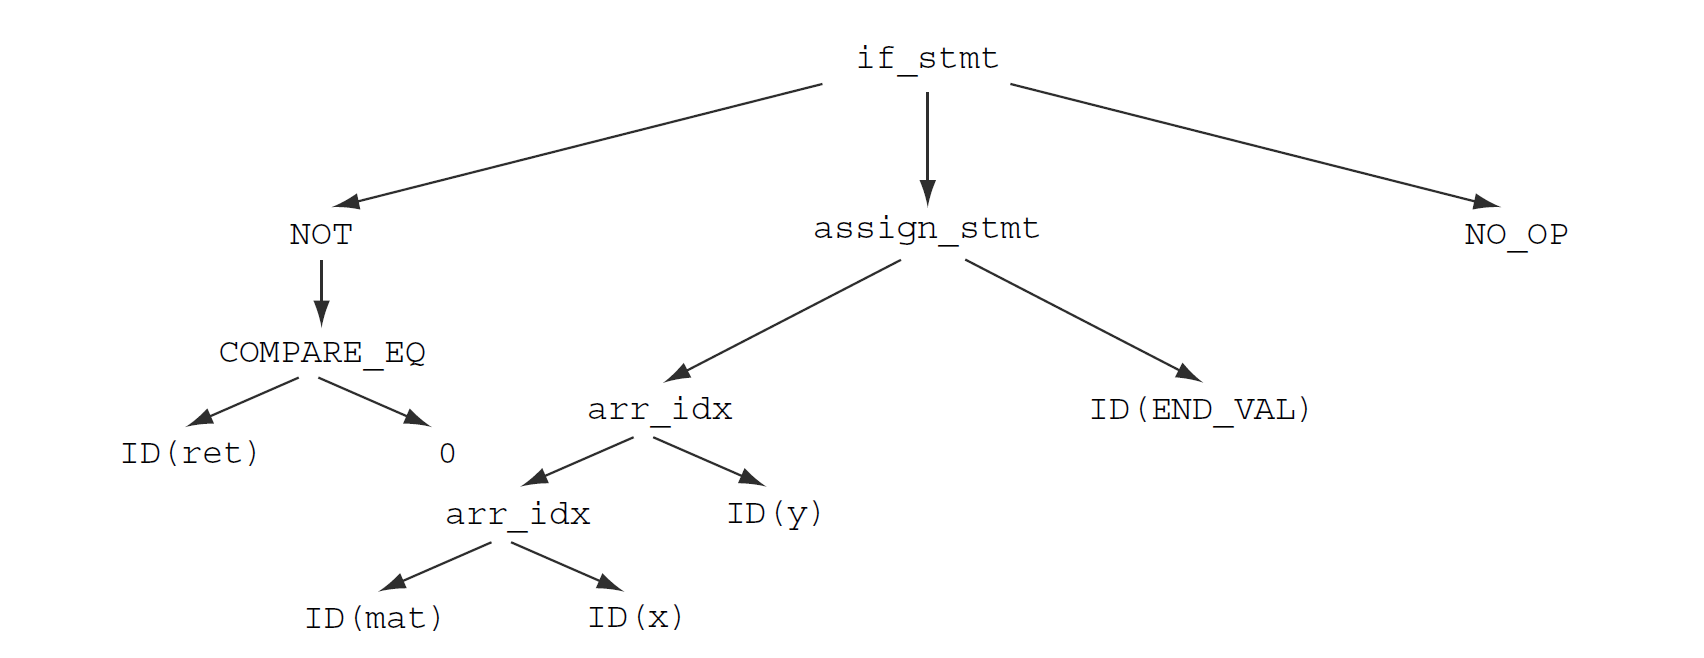
\includegraphics[width=1\textwidth]{Imagens/ArvoreAST}
		\label{fig:ArvoreAST}
		\caption{Árvore AST.}
	\end{figure}

	\section{Análise semântica}

	Como a AST está sendo construída, a ferramenta cria uma tabela de símbolos ao lado dela. Para cada identificador no programa, a tabela de símbolos associa o identificador com seu devido tipo e um ponteiro para a sua declaração ou definição. Com a AST e a tabela de símbolo, a ferramenta está agora equipado-se para realizar a verificação de tipo. A ferramenta de análise estática não pode ser obrigados a comunicar erros de checagem de tipo da maneira um compilador faz, mas informações de tipo é criticamente importante para a análise de uma linguagem orientada a objetos, porque o tipo de um objeto determina o conjunto de métodos que o objeto pode invocar. Além disso, é normalmente desejável para converter, pelo menos, as conversões do tipo implícito no código fonte para conversões de tipo explícitas no AST. Por estas razões, uma ferramenta de análise estática avançado tem a ver apenas como muito trabalho relacionado com a verificação de tipo como um compilador faz. No mundo do compilador, resolução de símbolo e verificação de tipo são referidos como análise semântica porque o compilador está atribuindo significado aos símbolos encontrada no programa. As ferramentas de análise estática que usam essas estruturas de dados têm uma vantagem distinta sobre ferramentas que não o fazem. Por exemplo, eles podem interpretar corretamente o significado dos operadores sobrecarregados em C++ ou determinar que um método em Java chamado doPost () é, na verdade, uma parte de uma implementação de HttpServlet.Estas capacidades permitem uma ferramenta para executar verificações úteis na estrutura deo programa. Após análise semântica, compiladores e a análise estática mais avançada ferramentas de formas de peça. Um compilador moderno usa a AST e o símbolo e o tipo informações para gerar uma representação intermediaria, uma versão genérico do código de máquina que é adequado para otimização e, em seguida, a conversão em específico da plataforma de código-objeto. O caminho para ferramentas de análise estática é menos clara. Dependendo do tipo de análise a ser realizada, uma ferramenta de análise estática pode executar transformações adicionais sobre a AST ou pode gerar a sua própria variedade de representação intermediária adequada às suas necessidades. Se uma ferramenta de análise estática usa sua própria representação intermediária, que, geralmente, permite a atribuição, pelo menos, ramificando, {\it looping}, e chamadas de função. A representação intermediária que uma ferramenta de análise estática usa é geralmente umvista de nível superior do programa do que a representação intermediária que um compilador usa. Por exemplo, um compilador de linguagem C, provavelmente, converter todas as referências a campos para estruturar deslocamentos em {\it byte} na estrutura pela sua representação intermediaria, enquanto uma ferramenta de análise estática mais provavelmente continuará para se referir a estrutura de campos, pelos seus nomes.\\

	\section {Checagem de tipo}
	
	A checagem de tipos é a forma mais utilizada de análise estática, e aquela que a maioria dos programadores estão familiarizados. As regras do "jogo" são tipicamente definida pela linguagem de programação e executadas pelo compilador, portanto, um programador que obtiver pouco a dizer quando a análise é executada ou como a análise funciona. Verificação de tipo elimina categorias inteiras de erros de programação. Por exemplo, ele impede programadores de atribuição acidentalmente valores integrais de oposição variáveis. Pela captura de erros em tempo de compilação, verificação de tipo de tempo de execução e impede erros. Verificação de tipo é limitado em sua capacidade de detectar erros, porém, sofre com falsos positivos e falsos negativos como todas as outras formas de análise estática. Curiosamente, os programadores raramente reclamar sobre uma escreva imperfeições do verificador. As demonstrações de Java no exemplo não vai compilar porque nunca é legal para atribuir uma expressão do tipo int para uma variável do tipo short, mesmo que a intenção do programador é inequívoca. A checagem de tipo sofre de falsos negativos também. Um exemplo de Java será quando o programa passará a verificação de tipo e compilar sem problemas, mas será falhar em tempo de execução. Arrays em Java são covariante, o que significa que o verificador de tipos permite uma variável de matriz de objeto para manter uma referência a uma matriz String (porque a classe String é derivado da classe de objecto), mas no tempo de execução Java não vai permitir que a matriz String para conter uma referência a um objeto do tipo Objeto.\\
	
	Um falso positivo de verificação de tipo: Estas declarações Java não satisfazem tipo regras de segurança, embora sejam logicamente correta.\\
	\begin{lstlisting}
	short s = 0;
	int i = s; /* o checador de tipos permite isso */
	short r = i; /*causara um falso positivo em tempo de compilacao assim ocorrendo um erro de tipo.*/
	\end{lstlisting}

	\section {Checagem de estilo}
	
	Verificadores de estilo também são ferramentas de análise estática. Eles geralmente impor um pickier e um conjunto de regras mais superficial do que um verificador de tipos. Verificadores puro estilo fazem cumprir as regras relacionadas com espaços em branco, nomeação, funções obsoletas, comentando, estrutura de programa, e semelhantes. Como muitos programadores estão ferozmente anexado a sua própria versão de um bom estilo, a maioria dos verificadores de estilo são bastante flexível sobre o conjunto de regras que impõem. Os erros produzidos pela verificadores estilo muitas vezes podem afetar a legibilidade e a manutenção do código, mas não indicam que um erro particular irá ocorrer quando o programa rodam. Com o tempo, alguns compiladores têm implementado verificações de estilo opcionais. Por exemplo, bandeira do gcc: -Wall fará com que o compilador para detectar quando um switch não leva em conta todos os valores possíveis de um {\it Enum} escrito.\\
	
	\section {Entendimento do código}
	
	Ferramentas do programa compreensão ajudam os programadores a entender o sentido  do programa de uma grande base de código. Os ambientes de desenvolvimento integrado (IDEs) incluem pelo menos algumas funcionalidade compreensão programa. Exemplos simples incluem "encontrar tudo utiliza desse método " e/ou " encontrar a declaração dessa variável global". Uma análise mais avançada pode suportar funcionalidades automáticas programa de refatoração, como renomear variáveis ou dividir uma única função em múltiplos funções. De nível superior ferramentas compreensão programa de tentar ajudar os programadores ter uma visão sobre a forma como um programa funciona. Alguns tentam fazer engenharia reversa informações sobre a concepção do programa com base em uma análise da implementação, dando assim o programador uma visão abrangente do programa. Isto é particularmente útil para programadores que precisam entender o programa fora de um grande corpo de código que eles não escreveram.\\
	
	\section {Verificação de programa}
	
	A verificação de programa é uma ferramenta que aceita uma especificação e um corpo de código e em seguida, as tentativas para demonstrar que o código é implementado fielmente com a especificação. A especificação é uma descrição completa de tudo o programa deveria fazer, a ferramenta de verificação de programa pode realizar equivalência verificar se o código e a especificação corresponder exatamente. Mais comumente as ferramentas de verificação de software contra um especificação parcial que detalha apenas uma parte do comportamento de um programa. Este esforço, por vezes, passa a verificação de propriedade de nome. A maioria das ferramentas de verificação tendem a trabalhar na aplicação de inferência lógica ou realizando verificação de modelos. Muitas ferramentas de verificação de propriedade concentram-se em propriedades de segurança temporais. A propriedade de segurança temporais especifica uma seqüência ordenada de eventos que um programa que não deve ser realizada. Um exemplo de uma propriedade de segurança temporal é. Um local de memória não deve ser lido depois de ser libertado." A maioria das ferramentas permitem aos programadores escrever suas próprias especificações para verificar as propriedades específicas do programa.\\
	
	\section {Verificação de propriedade}
	
	Uma ferramenta de verificação propriedade é dito ser de som com respeito à especificação se ele vai sempre relatar um problema se houver. Em outras palavras, a ferramenta nunca vai sofrer um falso negativo. A maioria das ferramentas que afirmam ser de som exigir que o programa que está sendo avaliado cumprir determinadas condições. Alguns não permitem ponteiros de função, enquanto outros não permitir recursão ou assumir que dois ponteiros nunca de alias (aponte para o mesmo local de memória). Para grandes quantidades de código, é quase impossível de satisfazer as condições estipuladas pela ferramenta, de modo a garantia de solidez não é significativo. Por esta razão, a solidez é raramente uma exigência do ponto de vista de um praticante.Em busca da solidez ou por causa de outras complicações, uma propriedade de verificação ferramenta pode produzir falsos positivos. No caso de um falso positivo, o contra-exemplo irá conter um ou mais eventos que não podia realmente ter lugar. Um exemplo é uma fuga de memória. O verificador de propriedade deu errado; ele não entende que, ao retornar NULL, malloc () é indicando que não há memória foi alocada. Isso pode indicar um problema com a forma como a propriedade for especificado,ou poderia ser um problema com o modo como o verificador propriedade funciona.